\chapter{Desenvolvimento Parcial} % TODO: Melhorar isso no futuro

Esta seção apresenta a etapa inicial de \textit{fine-tuning} do \ac{LLaMA}-3.2, sendo que ela tem um caráter exploratório e visa o desenvolvimento do código base para
os próximos Experimentos e também analisar a capacidade de classificação do modelo.

\section{Tecnologias Utilizadas}

O processamento de dados e \textit{fine-tuning} foram feitos com \textit{scripts} em Python e \textit{Jupyter notebooks}. As dependências do projeto foram gerenciadas
com o gerenciador Poetry e o \textit{framework} de \textit{fine-tuning} utilizado foi o Unsloth. Os treinamentos foram realizados com uma placa NVIDIA H100 de 80 GB, que
faz parte de uma plataforma NVIDIA DGX H100.

\section{Conjunto de Dados}

Inicialmente, o objetivo era começar os experimentos com imagens de aproximação e seus laudos provenientes do \ac{STT/SC}, porém, devido a uma demora na obtenção dos
dados, optou-se por utilizar temporariamente o conjunto de dados \ac{HAM10000}. Sendo assim, os experimentos inciais foram feitos com imagens de dermatoscopia.

O conjunto de dados é separado nas seções \textit{train}, \textit{test} e \textit{validation}, que possuem 9577, 1285 e 2492 imagens, respectivamente. A
\autoref{tab:ham10000_proportion} apresenta as proporções entre as lesões de pele. Os dados foram obtidos a partir da plataforma Hugging Face com uma versão do
\ac{HAM10000} fornecida por \textcite{skin_cancer_dataset}.

\begin{table}[ht]
    \caption{\small Proporção entre as diferentes categorias de lesões de pele no \ac{HAM10000}.}
    \centering
    \begin{tabular}{l|c}
        \hline
        Lesão de pele                        & Proporção (\%) \\ \hline
        Nevo melanocítico                    & 66,88          \\
        Melanoma                             & 11,23          \\
        Lesões similares à queratose benigna & 10,94          \\
        CBC                                  & 5,08           \\
        Queratose actínica                   & 3,29           \\
        Lesões vasculares                    & 1,42           \\
        Dermatofibroma                       & 1,15           \\ \hline
    \end{tabular}
    \label{tab:ham10000_proportion}
    \fonte{\textcite{tschandl2018ham10000}}
\end{table}

\section{Experimentos com \textit{Fine-tuning}}

Os experimentos utilizaram a variante \ac{LLaMA}-3.2-11B-Vision-Instruct, que possui 11 bilhões de parâmetros. Os métodos de \textit{fine-tuning} utilizados foram o
\ac{LoRA} e o \ac{QLoRA}.

\subsection{Dados de treinamento}

O modelo utilizado não suporta ainda a utilização de textos em português para tarefas multimodais, sendo assim, os diálogos estão em inglês. Foi aplicada uma amostragem
estratificada por categoria de lesão de pele sobre os dados de treinamento para que os diálogos tivessem uma representação proporcional de cada lesão de pele. Eles
possuem o seguinte formato:

\begin{dialogue}
    \speak{Usuário} \textit{Classify the skin lesion in the image. \textbf{<imagem>}} \\
    \speak{Modelo} \textit{The skin lesion in the image is \textbf{<lesão de pele>}.}
\end{dialogue}

\subsection{\textit{Fine-tuning} com 450, 900 e 1800 amostras}

% TODO: Ver se é necessário citar os criadores do Adam e AdamW.

A primeira etapa nos experimentos realizar o \textit{fine-tuning} com \ac{QLoRA} com 450 amostras de treinamento e 50 de validação. Os hiperparâmetros\footnote{parâmetros
    de treinamento} utilizados no treinamento estão na \autoref{tab:qlora_500_config}, alguns deles foram omitidos por serem menos relevantes nessa etapa. O \ac{rsLoRA} de
\textcite{kalajdzievski2023rank} foi utilizado para melhorar o desempenho, utilizando um fator de escala \begin{math}\frac{\alpha_{LoRA}}{\sqrt{r}}\end{math} em vez do
\begin{math}\frac{\alpha_{LoRA}}{r}\end{math} do \ac{LoRA} original. Por fim, também foi utilizado o otimizador \ac{Adam} na sua versão paginada de 32 bits. A
\autoref{tab:qlora_500_training} apresenta alguns dados sobre o treinamento e a \autoref{fig:loss_qlora_500} apresenta o \textit{loss} de treinamento e validação ao
longo dos passos.

\begin{table}[ht]
    \caption{\small Hiperparâmetros para o \ac{QLoRA} com 450, 900 e 1800 amostras. A primeira seção se refere às configurações específicas de \ac{PEFT}, enquanto a
    segunda se refere ao treinamento em geral.}
    \centering
    \begin{tabular}{l|c}
        \hline
        Hiperparâmetro                             & Valor                                  \\ \hline
        Camadas e módulos treinados                & Visão, linguagem, atenção e \ac{MLP}   \\
        Rank                                       & 32                                     \\
        Alfa (\begin{math}\alpha_{LoRA}\end{math}) & 32                                     \\
        Dropout                                    & 0,1                                    \\
        \ac{rsLoRA}                                & Sim                                    \\ \hline
        Taxa de aprendizado                        & \begin{math}2 \times 10^{-4}\end{math} \\
        Razão de aquecimento                       & 0,03                                   \\
        Tipo de escalonador da taxa de aprendizado & Cosseno com reinícios                  \\
        Decaimento de peso                         & 0,01                                   \\
        Épocas                                     & 5                                      \\
        Passos a cada validação                    & 50                                     \\
        Otimizador                                 & \ac{Adam} paginado de 32 bits          \\
        Tipo numérico                              & \ac{BF16}                              \\ \hline
    \end{tabular}
    \label{tab:qlora_500_config}
    \fonte{Autoria própria}
\end{table}

\clearpage

\begin{table}[ht]
    \caption{\small Dados sobre o treinamento com \ac{QLoRA} com 450 amostras.}
    \centering
    \begin{tabular}{l|c}
        \hline
                                    & Valor     \\ \hline
        Parâmetros treináveis       & 134348800 \\
        Tempo de treinamento (min)  & 16,17     \\
        Passos                      & 110       \\
        Memória máxima alocada (GB) & 18.69     \\ \hline
    \end{tabular}
    \label{tab:qlora_500_training}
    \fonte{Autoria própria}
\end{table}

\begin{figure}[ht]
    \centering
    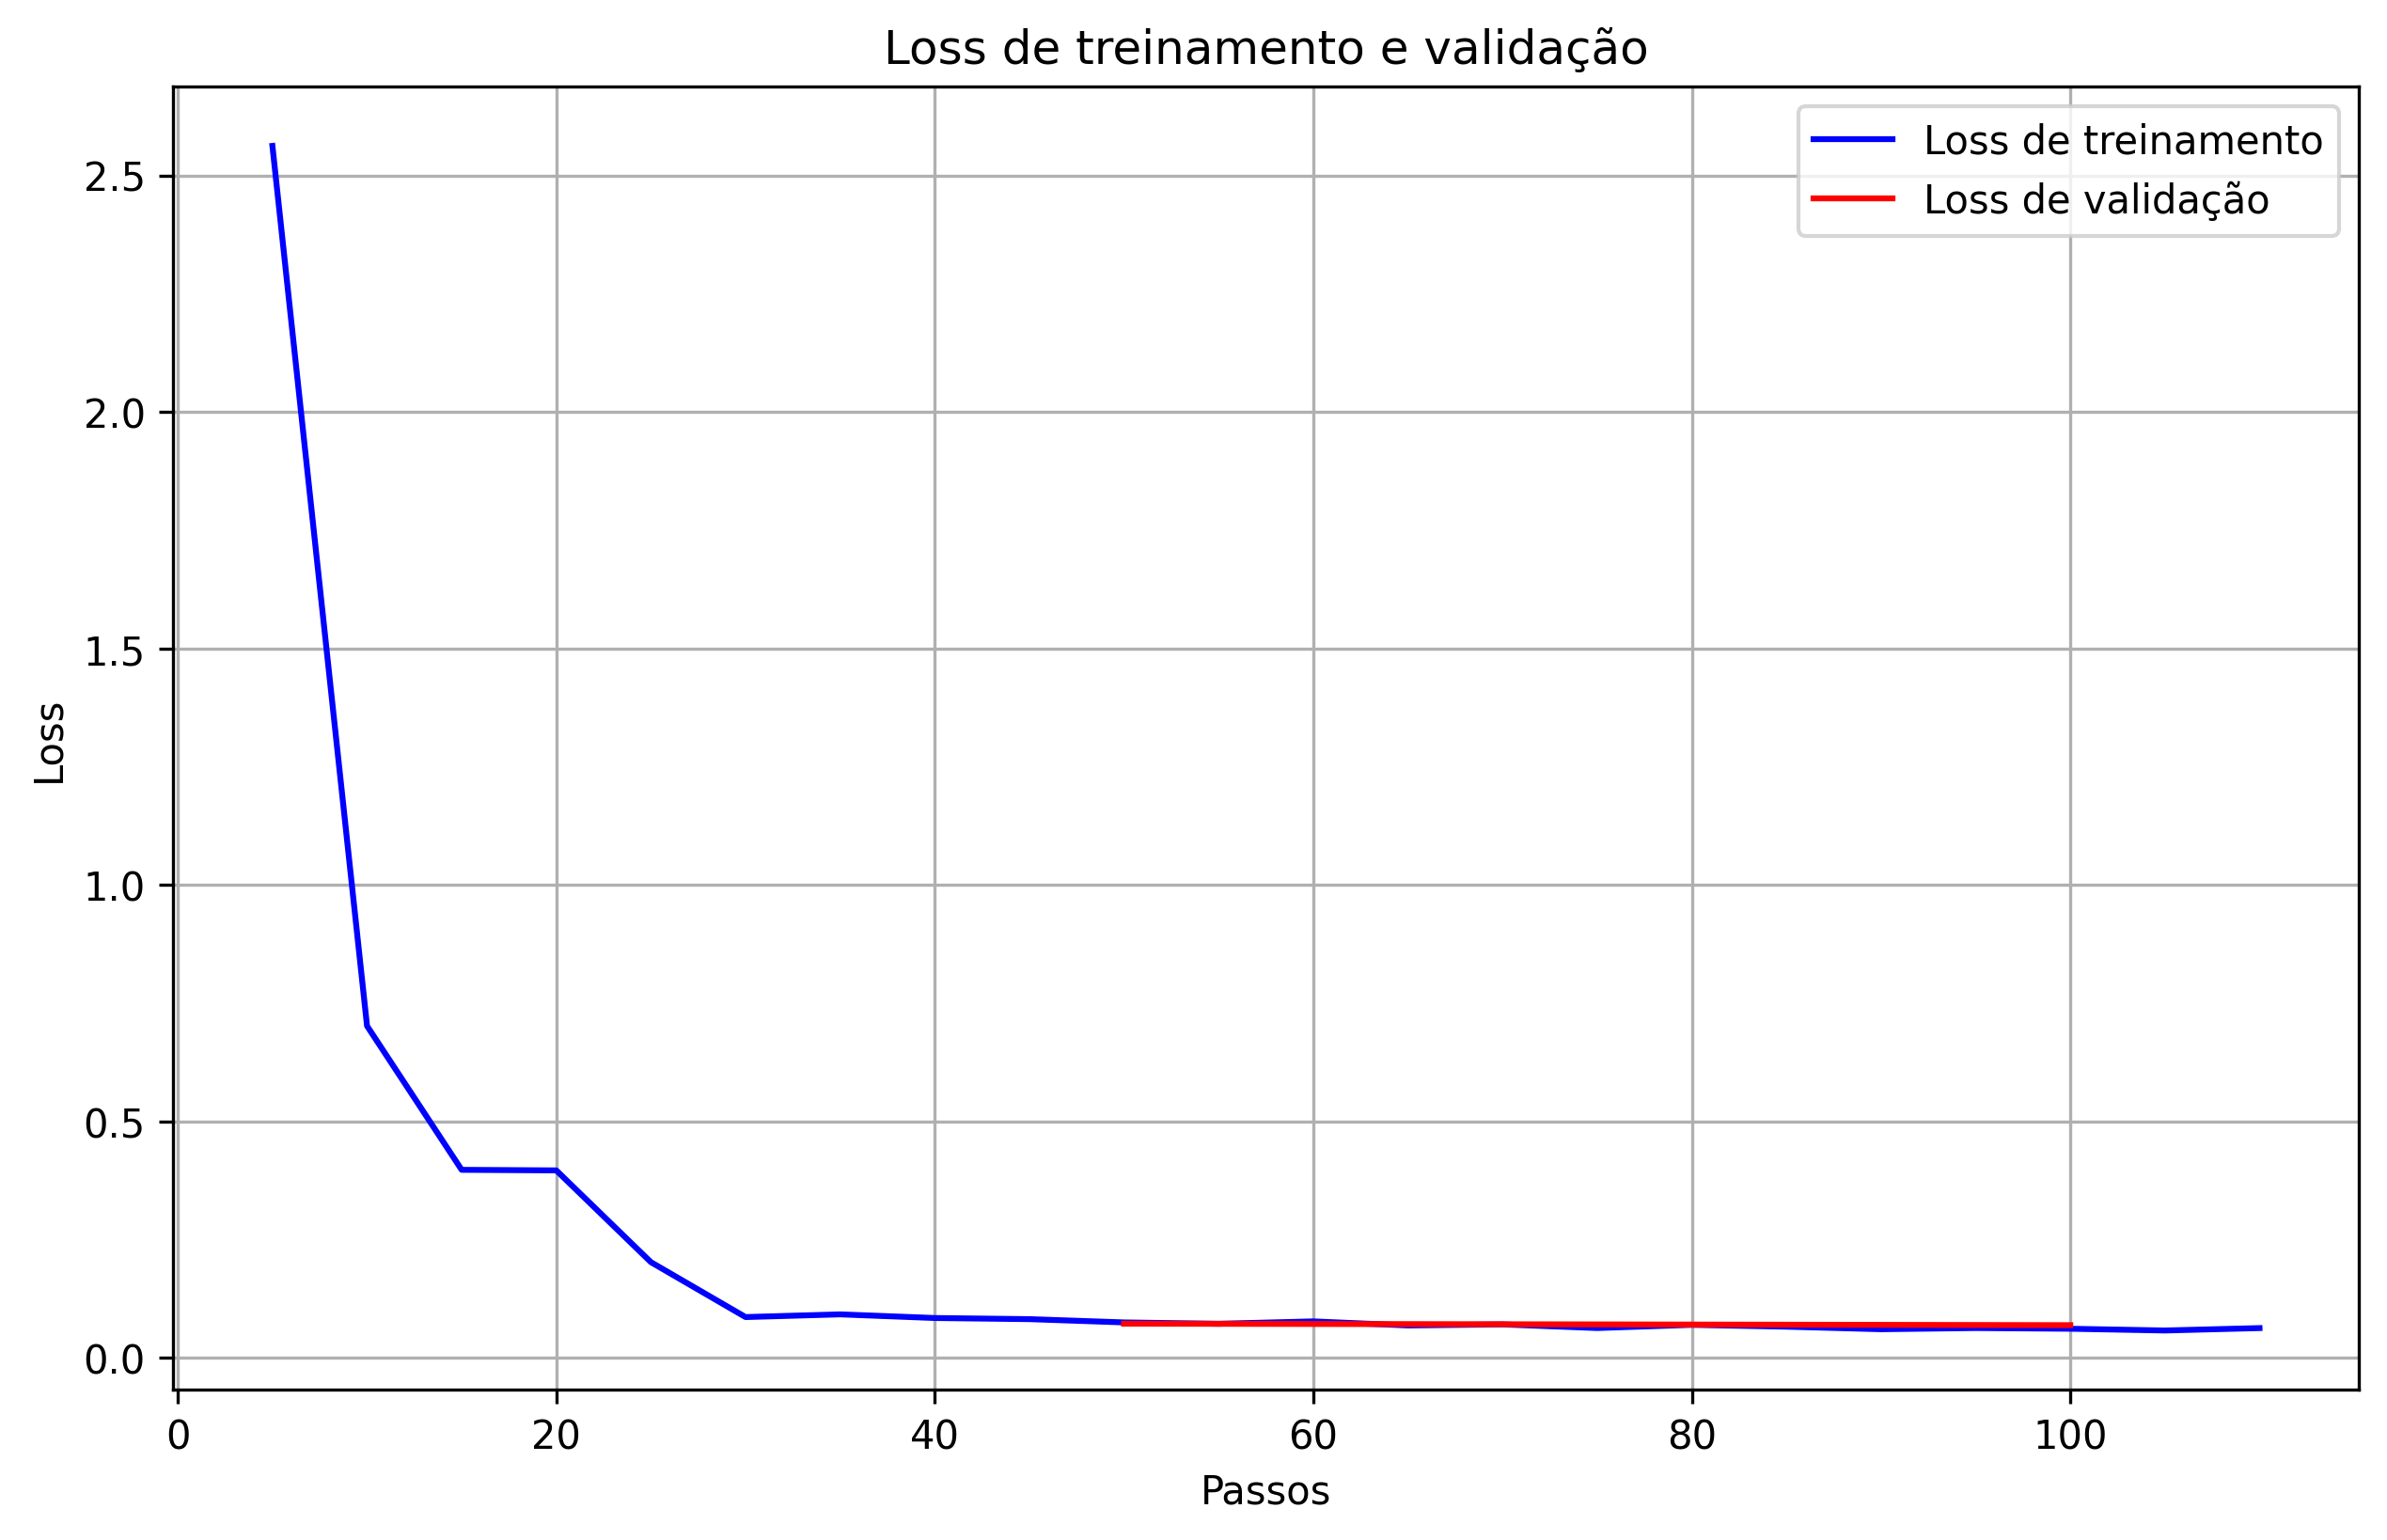
\includegraphics[width=0.8\columnwidth,keepaspectratio]{images/loss_qlora_500.png}
    \caption{\small \textit{Loss} de treinamento e validação para o \ac{QLoRA} com 450 amostras. Fonte: Autoria própria.}
    \label{fig:loss_qlora_500}
\end{figure}

Em seguida, foi realizado o \textit{fine-tuning} com \ac{LoRA}, ou seja, sem quantização, com 450 amostras. Os hiperparâmetros utilizados são similares, porém, o
\textit{rank} foi reduzido para 16, assim como o \begin{math}\alpha_{LoRA}\end{math}. O \ac{rsLoRA} não foi utilizado e a taxa de aprendizado foi reduzida a
\begin{math}1 \times 10^{-4}\end{math}. Por fim o otimizador \ac{AdamW} foi utilizado. A \autoref{tab:lora_500_training} apresenta os dados de treinamento e a
\autoref{fig:loss_lora_500} apresenta o \textit{loss}. O treinamento foi aplicado somente sobre 64174400 parâmetros, uma quantidade menor do que a usada no
\ac{QLoRA} por conta do \textit{rank} reduzido.

\begin{table}[ht]
    \caption{\small Dados sobre o treinamento com \ac{LoRA} com 450 amostras.}
    \centering
    \begin{tabular}{l|c}
        \hline
                                    & Valor    \\ \hline
        Parâmetros treináveis       & 64174400 \\
        Tempo de treinamento (min)  & 26,42    \\
        Passos                      & 140      \\
        Memória máxima alocada (GB) & 40,35    \\ \hline
    \end{tabular}
    \label{tab:lora_500_training}
    \fonte{Autoria própria}
\end{table}

\clearpage

\begin{figure}[ht]
    \centering
    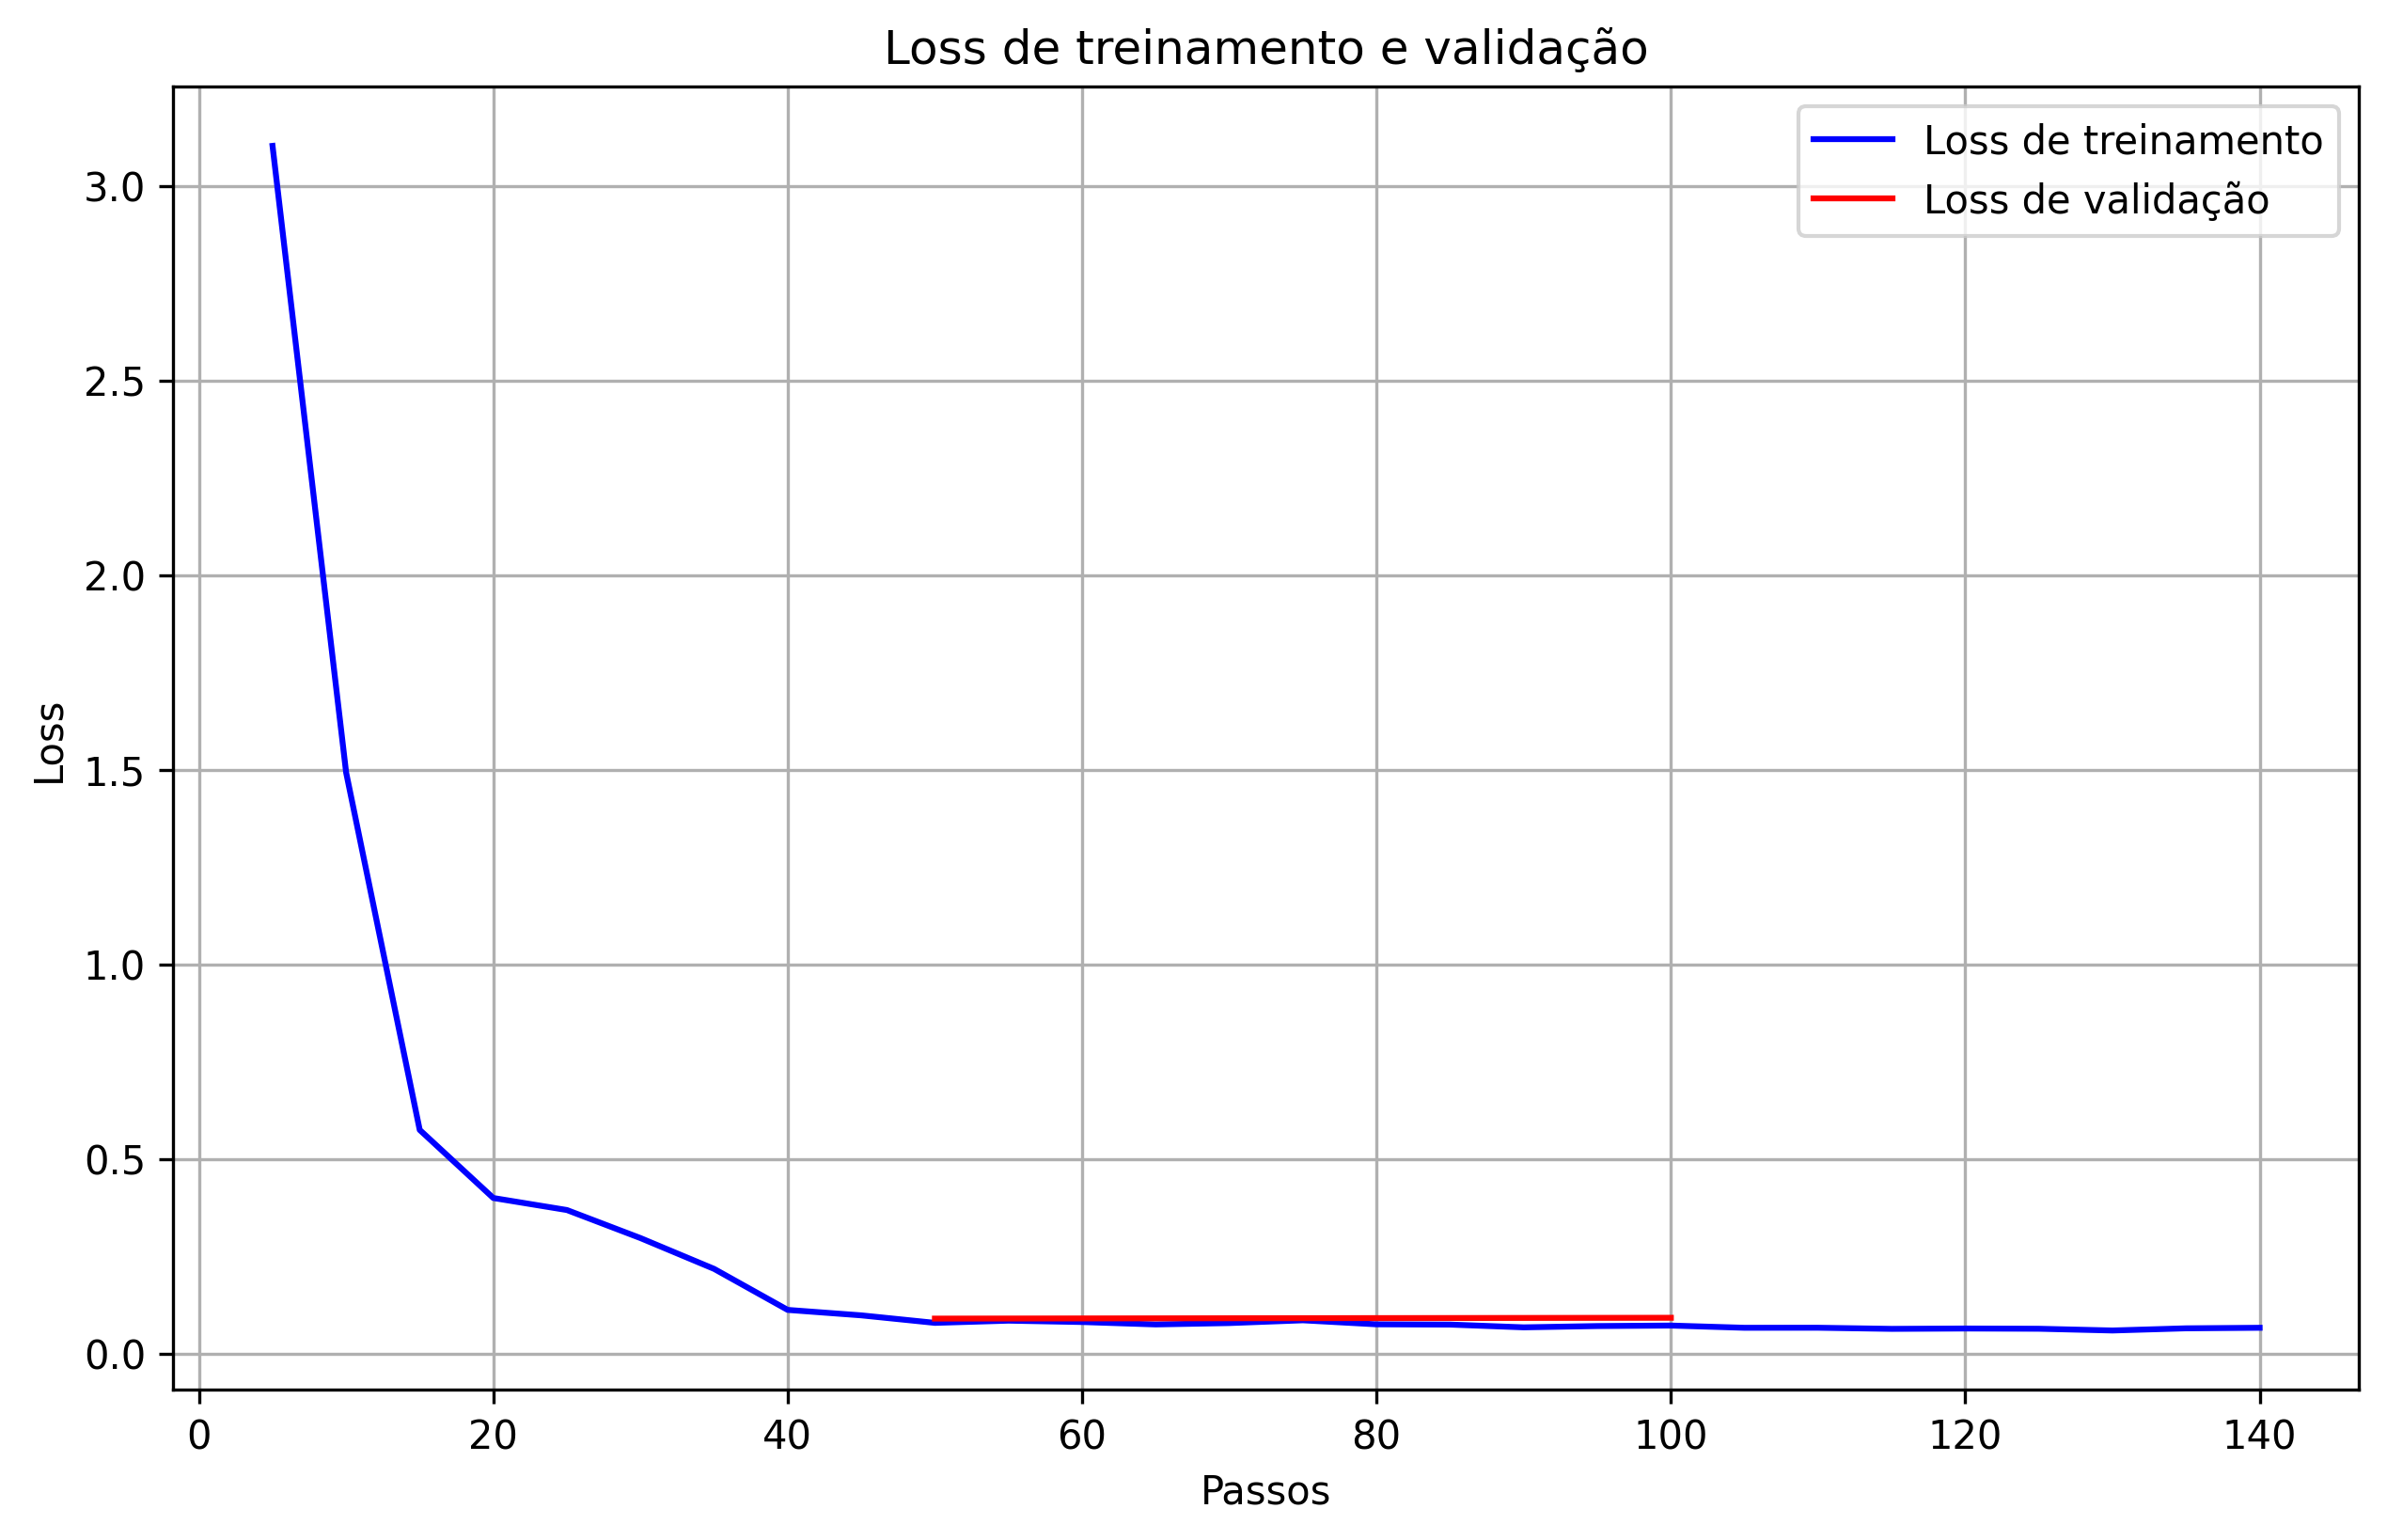
\includegraphics[width=0.725\columnwidth,keepaspectratio]{images/loss_lora_500.png}
    \caption{\small \textit{Loss} de treinamento e validação para o \ac{LoRA} com 450 amostras. Fonte: Autoria própria.}
    \label{fig:loss_lora_500}
\end{figure}

O \textit{fine-tuning} com 900 amostras foi feito sem a alteração nos hiperparâmetros do \ac{QLoRA} e \ac{LoRA}. As informações sobre o treinamento podem ser conferidas
na \autoref{tab:qlora_1000_training} e \autoref{tab:lora_1000_training}, enquanto o \textit{loss} pode ser conferido na \autoref{fig:loss_qlora_1000} e
\autoref{fig:loss_lora_1000}.

\begin{table}[ht]
    \caption{\small Dados sobre o treinamento com \ac{QLoRA} com 900 amostras.}
    \centering
    \begin{tabular}{l|c}
        \hline
                                    & Valor     \\ \hline
        Parâmetros treináveis       & 134348800 \\
        Tempo de treinamento (min)  & 32,08     \\
        Passos                      & 225       \\
        Memória máxima alocada (GB) & 18,695    \\ \hline
    \end{tabular}
    \label{tab:qlora_1000_training}
    \fonte{Autoria própria}
\end{table}

\begin{table}[ht]
    \caption{\small Dados sobre o treinamento com \ac{LoRA} com 900 amostras.}
    \centering
    \begin{tabular}{l|c}
        \hline
                                    & Valor    \\ \hline
        Parâmetros treináveis       & 67174400 \\
        Tempo de treinamento (min)  & 41,76    \\
        Passos                      & 280      \\
        Memória máxima alocada (GB) & 31,965   \\ \hline
    \end{tabular}
    \label{tab:lora_1000_training}
    \fonte{Autoria própria}
\end{table}

\clearpage

\begin{figure}[ht]
    \centering
    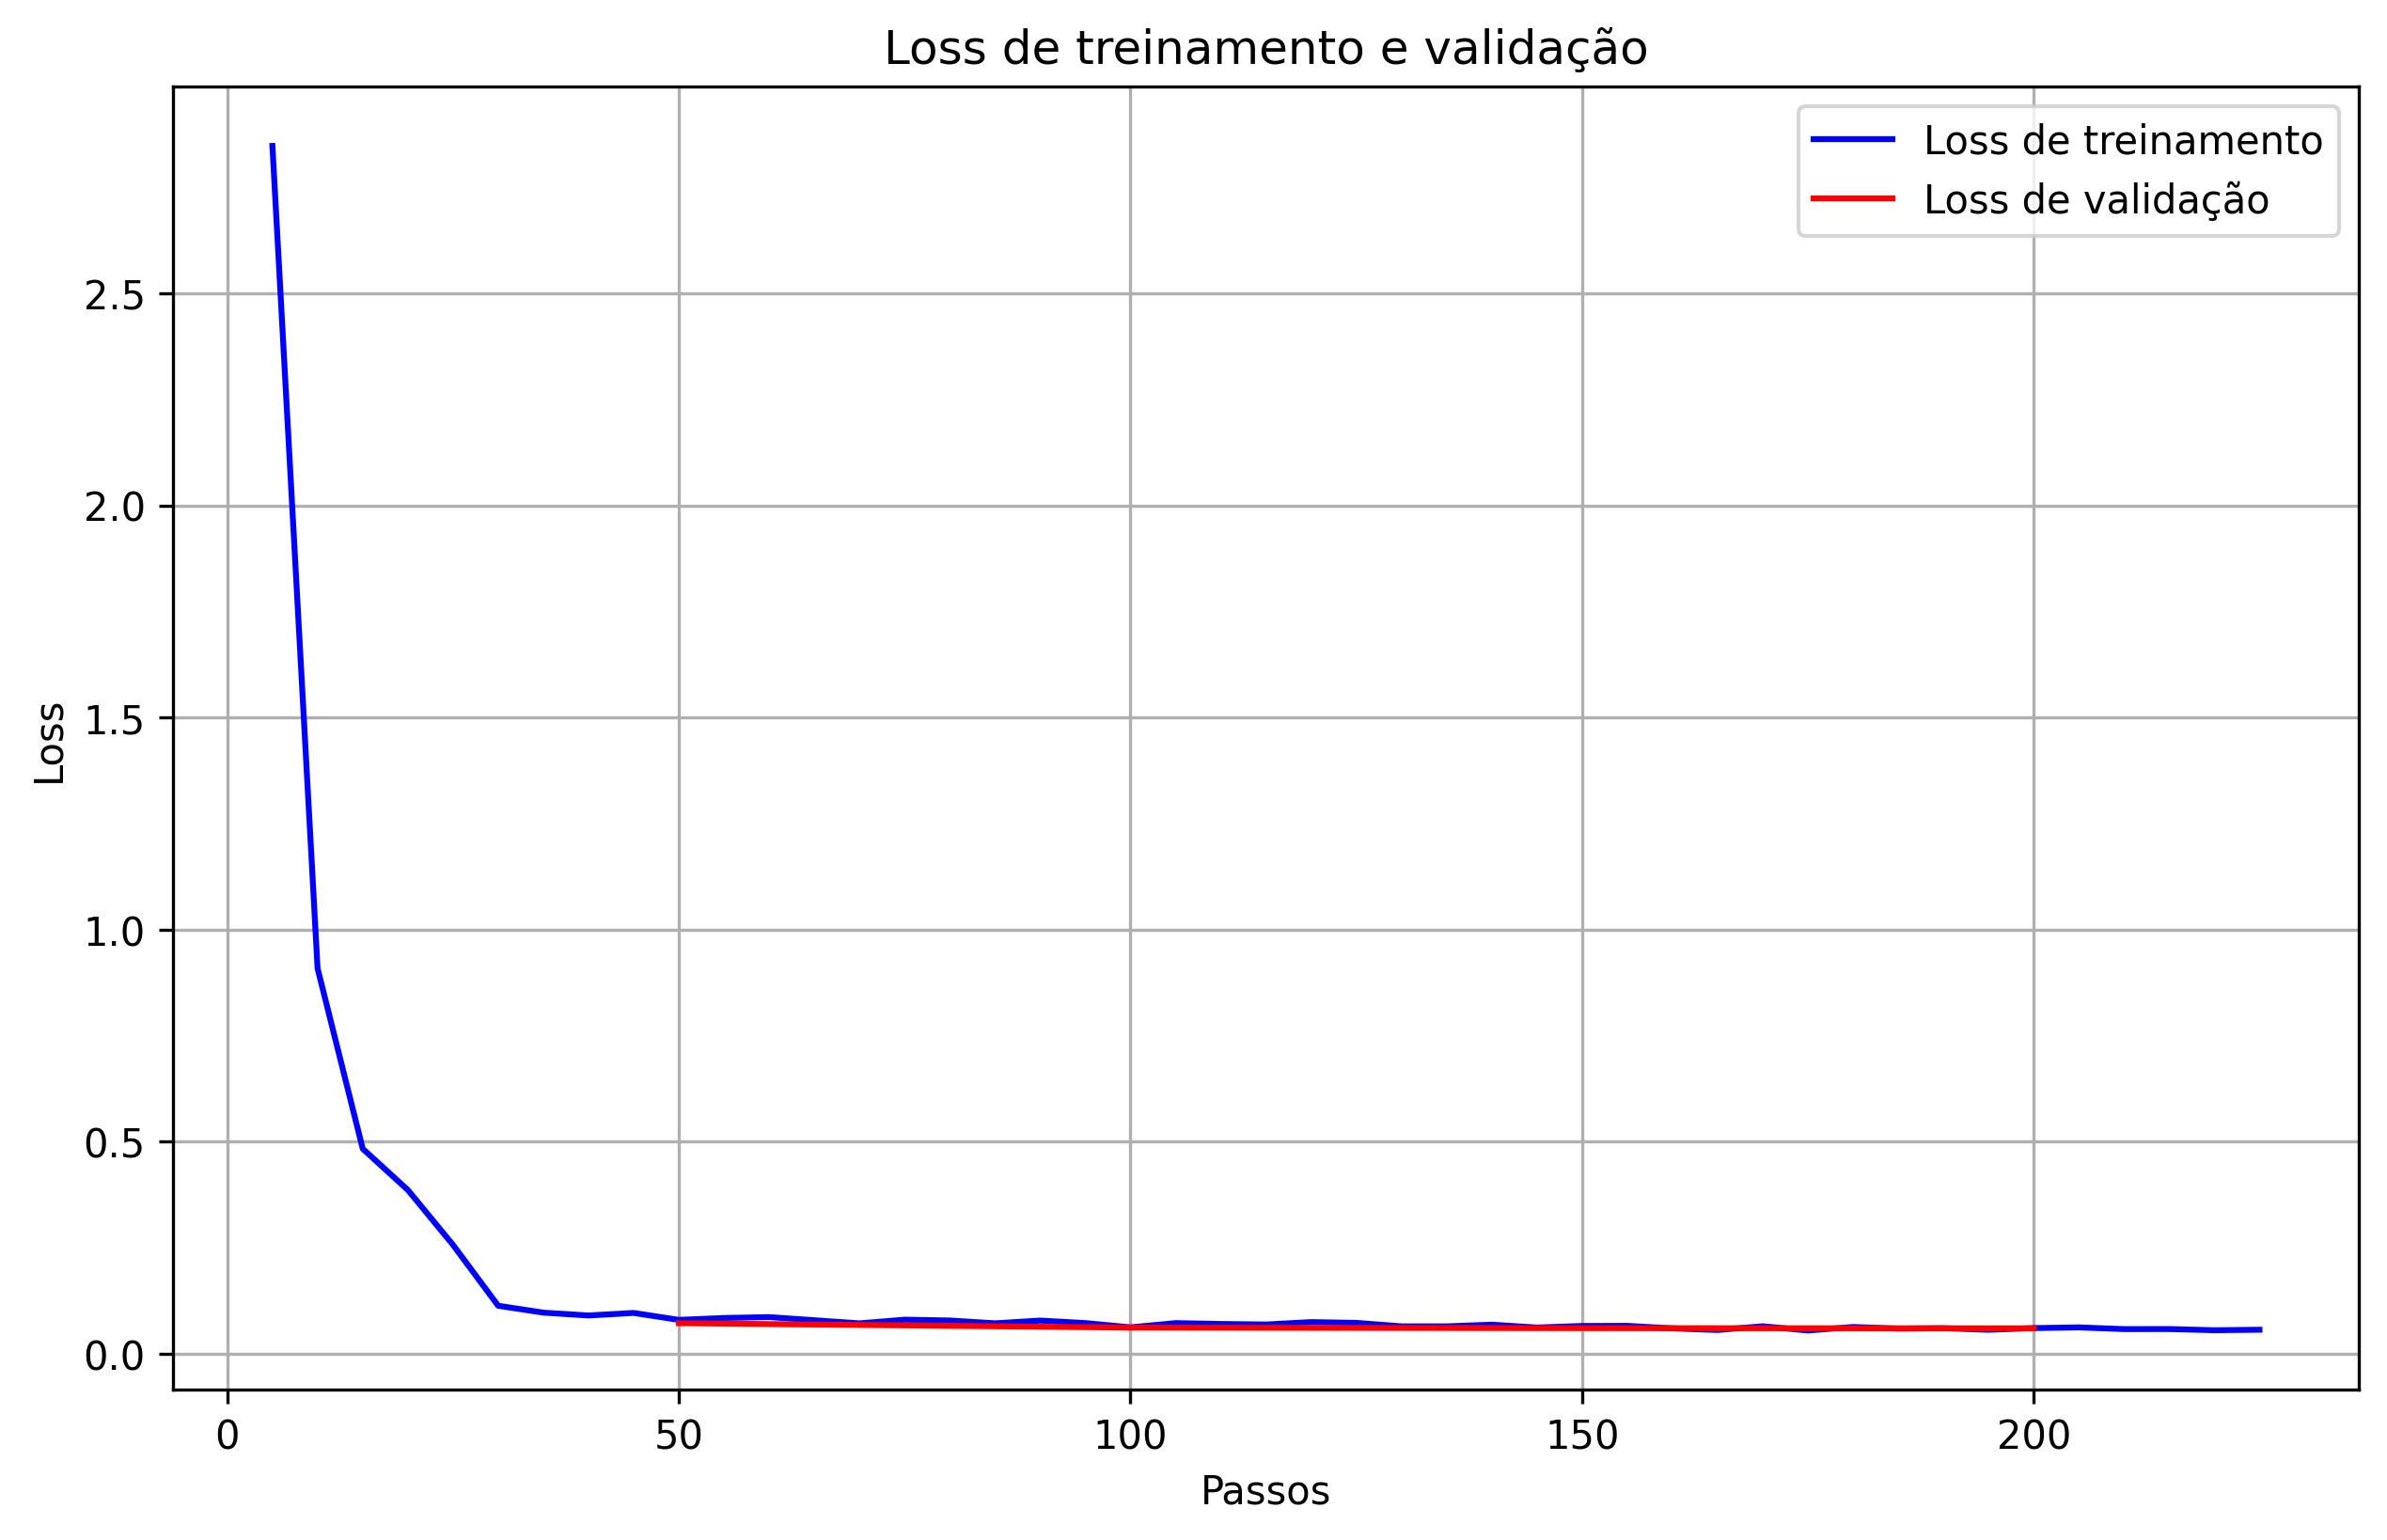
\includegraphics[width=0.725\columnwidth,keepaspectratio]{images/loss_qlora_1000.png}
    \caption{\small \textit{Loss} de treinamento e validação para o \ac{QLoRA} com 900 amostras. Fonte: Autoria própria.}
    \label{fig:loss_qlora_1000}
\end{figure}

\begin{figure}[ht]
    \centering
    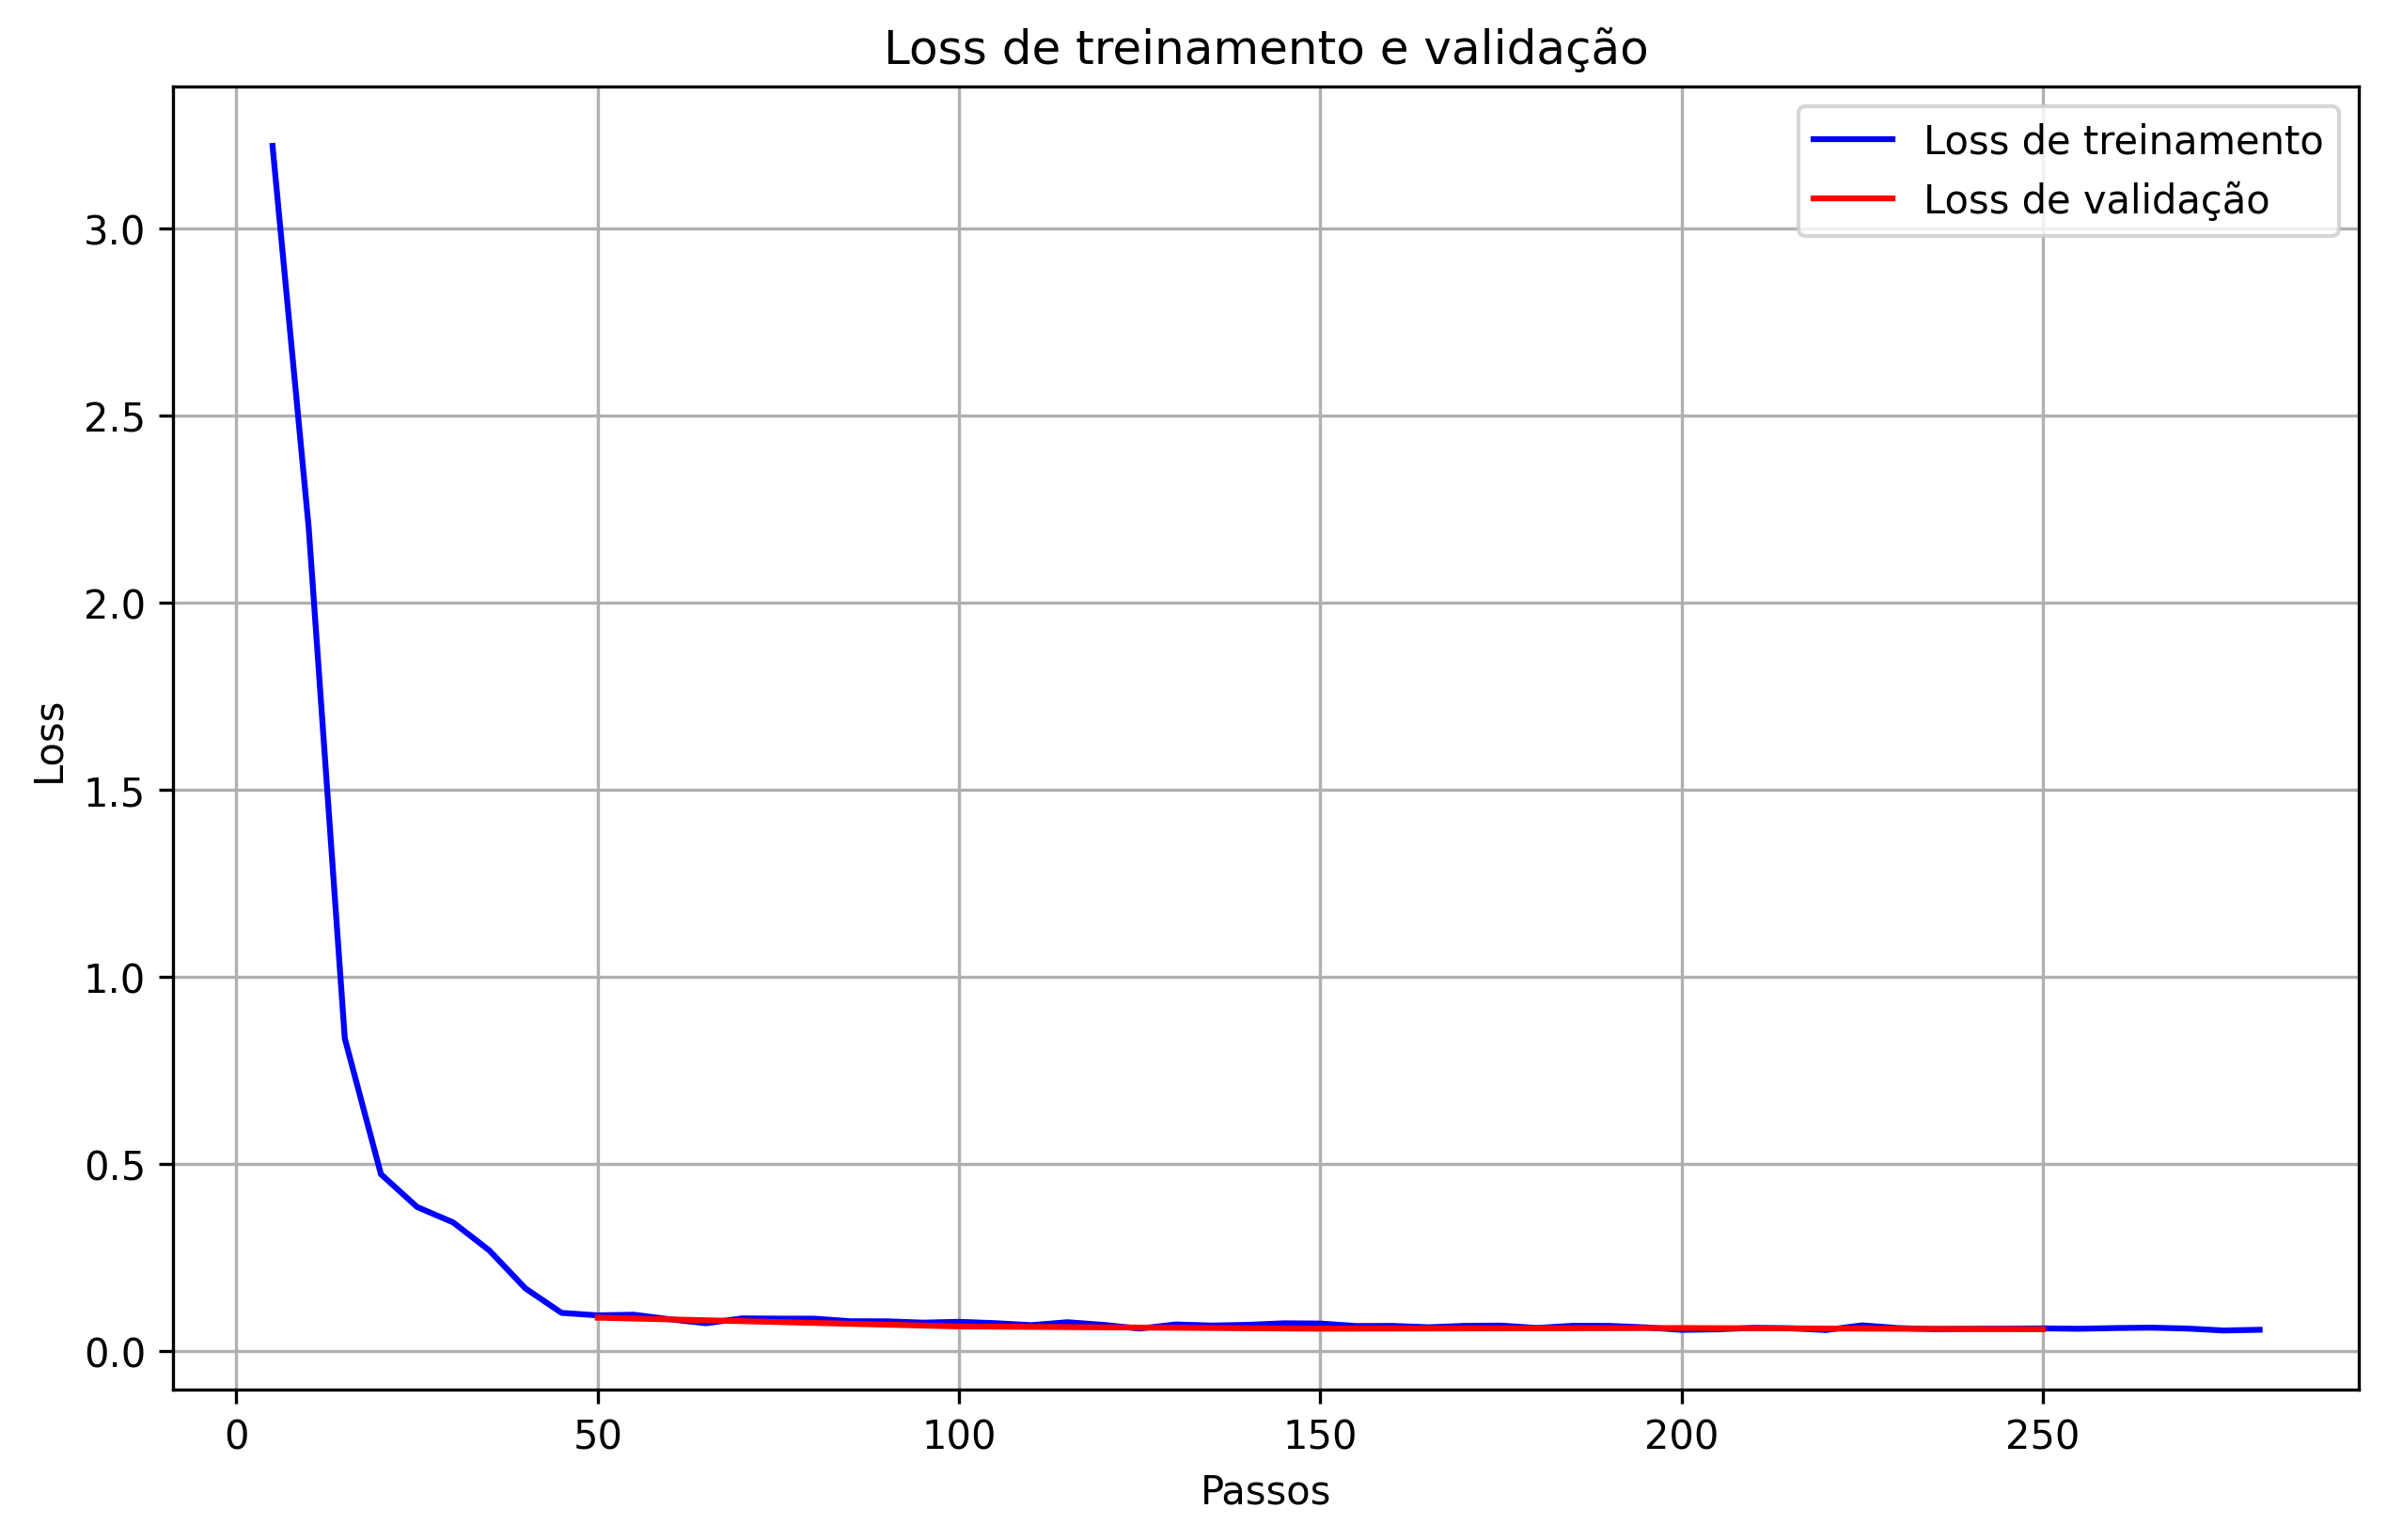
\includegraphics[width=0.725\columnwidth,keepaspectratio]{images/loss_lora_1000.png}
    \caption{\small \textit{Loss} de treinamento e validação para o \ac{LoRA} com 900 amostras. Fonte: Autoria própria.}
    \label{fig:loss_lora_1000}
\end{figure}

Por último, foi feito um \textit{fine-tuning} com \ac{QLoRA} com 1800 amostras com os mesmos hiperparâmetros utilizados anteriormente.

\clearpage

\begin{table}[ht]
    \caption{\small Dados sobre o treinamento com \ac{QLoRA} com 1800 amostras.}
    \centering
    \begin{tabular}{l|c}
        \hline
                                    & Valor     \\ \hline
        Parâmetros treináveis       & 134348800 \\
        Tempo de treinamento (min)  & 90,77     \\
        Passos                      & 450       \\
        Memória máxima alocada (GB) & 18,744    \\ \hline
    \end{tabular}
    \label{tab:qlora_2000_training}
    \fonte{Autoria própria}
\end{table}

\begin{figure}[ht]
    \centering
    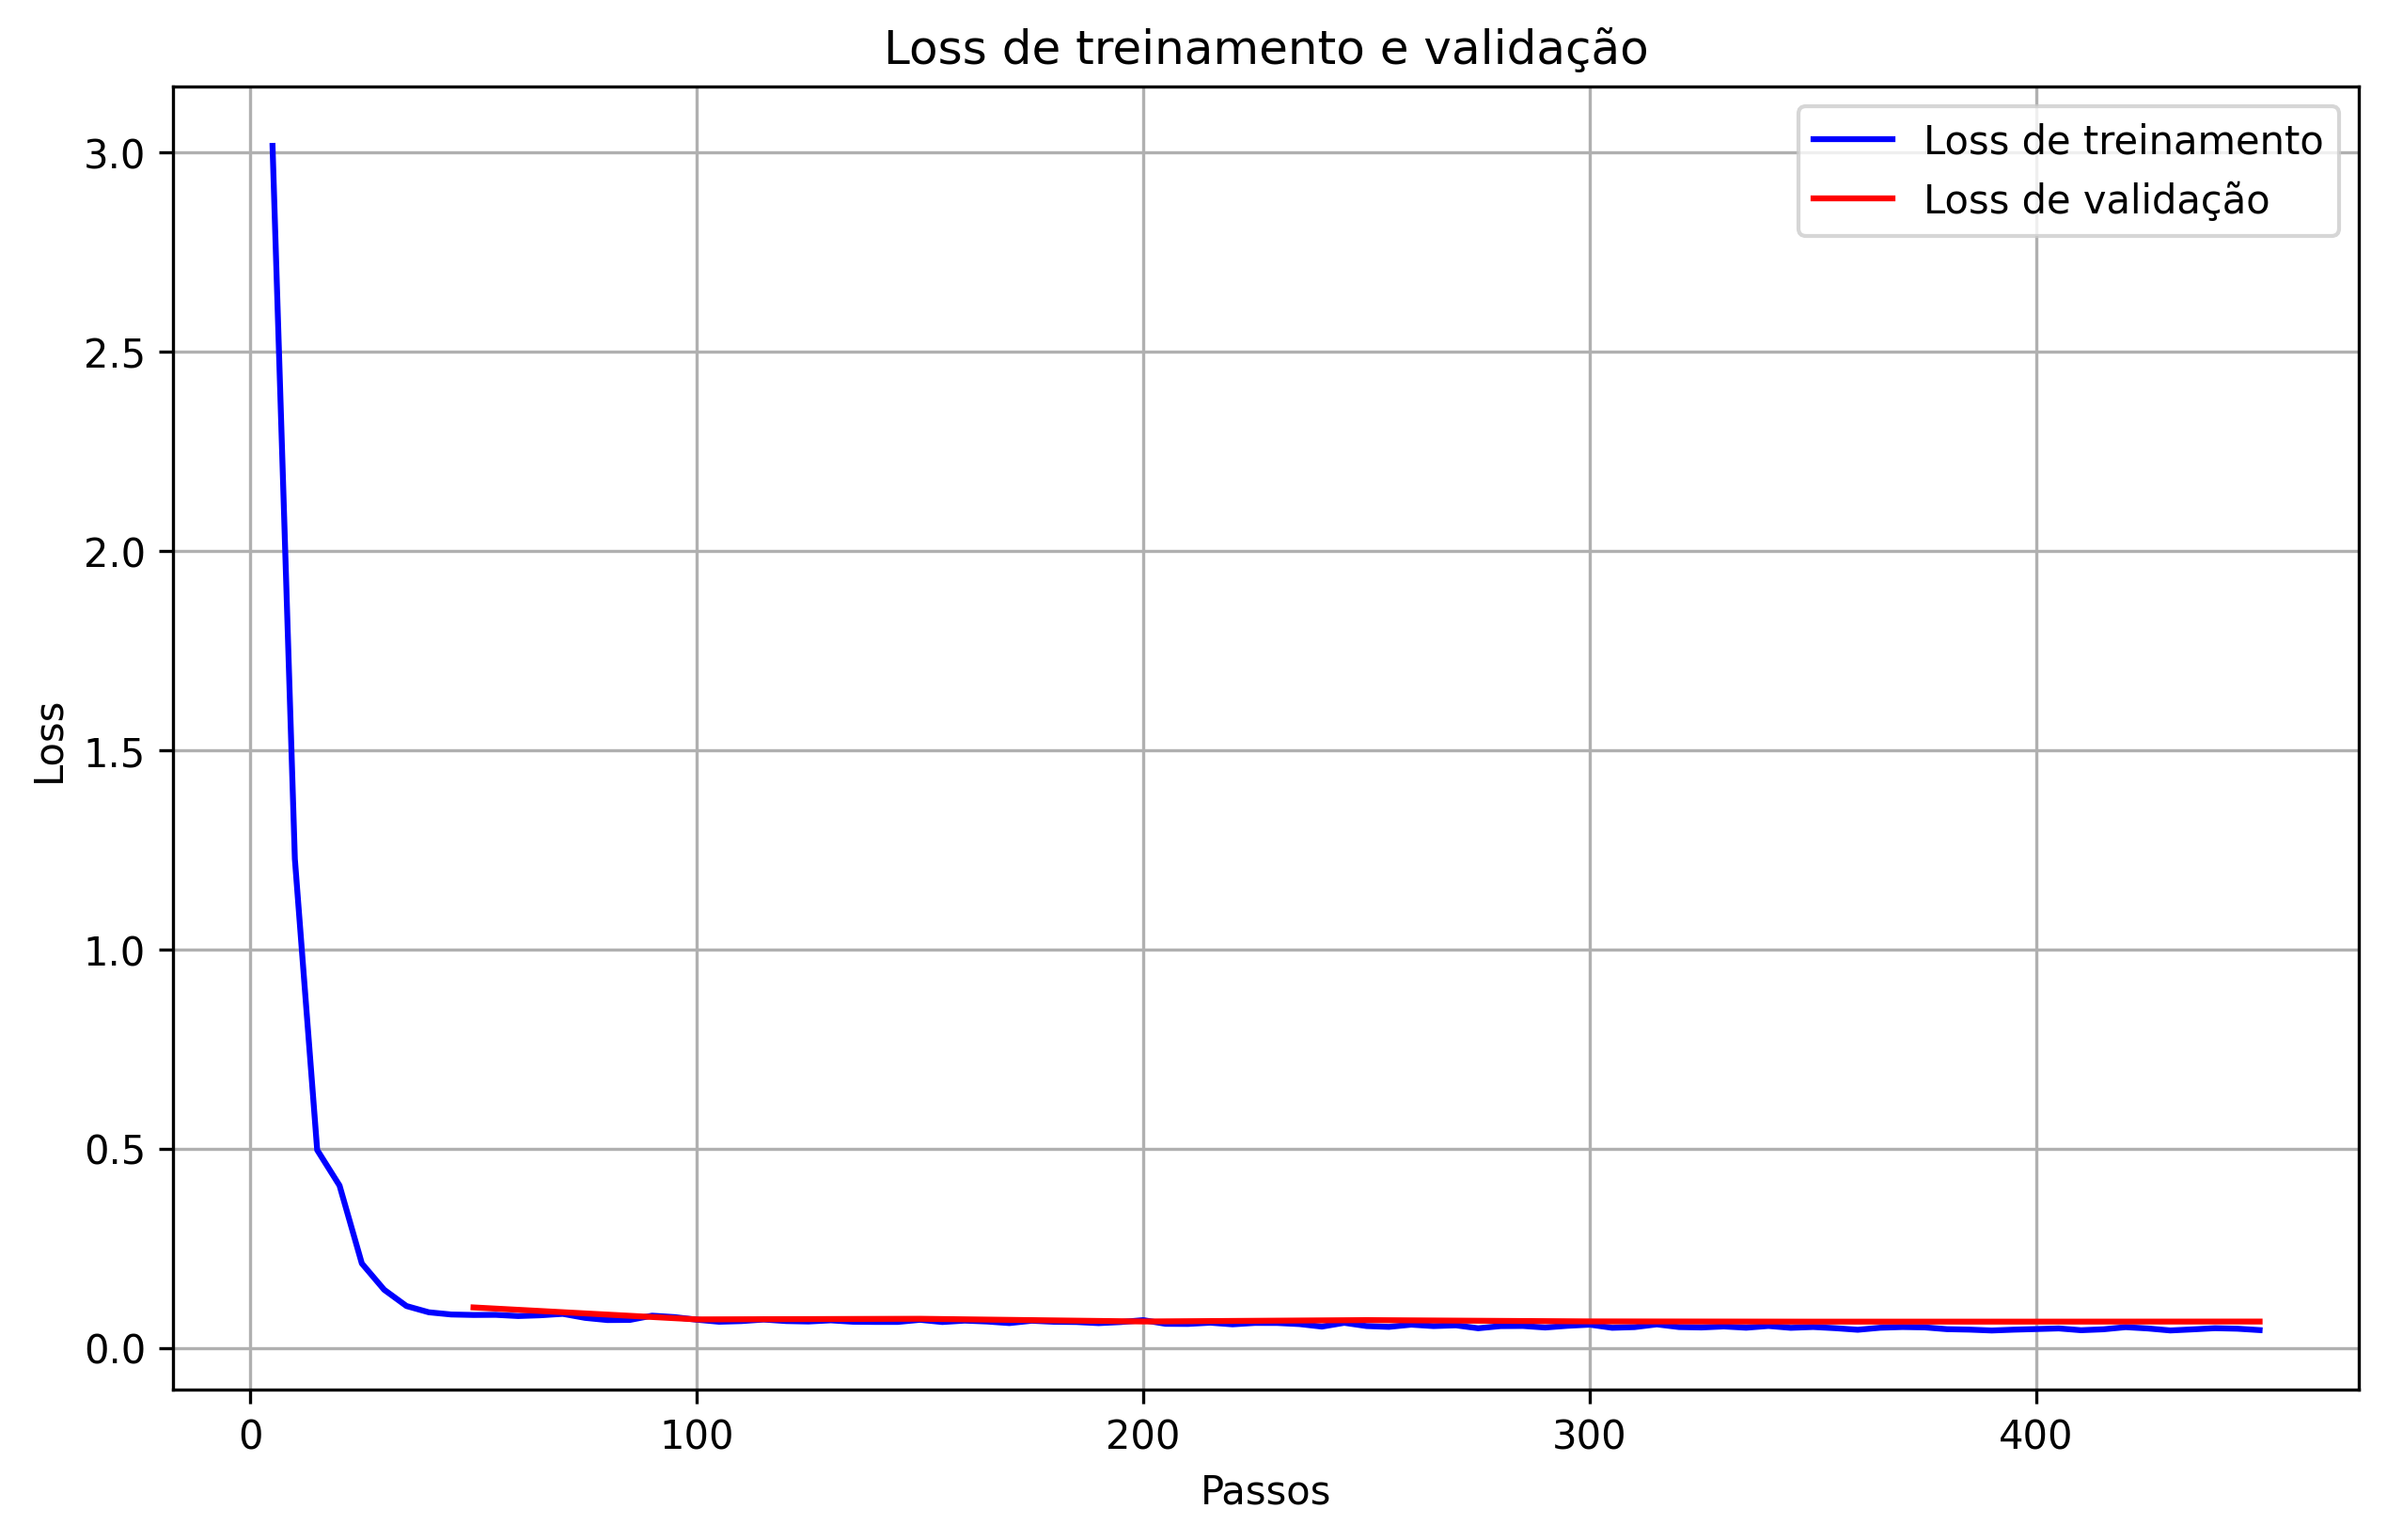
\includegraphics[width=0.725\columnwidth,keepaspectratio]{images/loss_qlora_2000.png}
    \caption{\small \textit{Loss} de treinamento e validação para o \ac{QLoRA} com 1800 amostras. Fonte: Autoria própria.}
    \label{fig:loss_qlora_2000}
\end{figure}

\subsection{\textit{Fine-tuning} com 5000 e 9500 amostras}

Para avaliar o impacto diferentes hiperparâmetros, foram feitos \textit{fine-tunings} modificados com 5000 e 9500 amostras. As configurações na
\autoref{tab:qlora_5000_config} se referem tanto ao \ac{QLoRA} quanto ao \ac{LoRA}. Foi utilizado somente o \ac{QLoRA} no treinamento com 9500 amostras. Os dados dos
treinamentos podem ser conferidos na \autoref{tab:qlora_5000_training}, \autoref{tab:lora_5000_training} e \autoref{tab:qlora_9500_training}, enquanto o \textit{loss}
pode ser conferido na \autoref{fig:loss_qlora_5000}, \autoref{fig:loss_lora_5000} e \autoref{fig:loss_qlora_9500}.

\clearpage

\begin{table}[ht]
    \caption{\small Hiperparâmetros para o \textit{fine-tuning} com 5000 amostras. A primeira seção se refere às configurações específicas de \ac{PEFT}, enquanto a
    segunda se refere ao treinamento em geral.}
    \centering
    \begin{tabular}{l|c}
        \hline
        Hiperparâmetro                             & Valor                                  \\ \hline
        Camadas e módulos treinados                & Visão, linguagem, atenção e \ac{MLP}   \\
        Rank                                       & 64                                     \\
        Alfa (\begin{math}\alpha_{LoRA}\end{math}) & 64                                     \\
        Dropout                                    & 0,05                                   \\
        \ac{rsLoRA}                                & Sim                                    \\ \hline
        Taxa de aprendizado                        & \begin{math}1 \times 10^{-4}\end{math} \\
        Razão de aquecimento                       & 0                                      \\
        Tipo de escalonador da taxa de aprendizado & Constante                              \\
        Decaimento de peso                         & 0,01                                   \\
        Épocas                                     & 3                                      \\
        Passos a cada validação                    & A cada 5\% dos passos                  \\
        Otimizador                                 & \ac{Adam} paginado de 32 bits          \\
        Tipo numérico                              & \ac{BF16}                              \\ \hline
    \end{tabular}
    \label{tab:qlora_5000_config}
    \fonte{Autoria própria}
\end{table}

\begin{table}[ht]
    \caption{\small Dados sobre o treinamento com \ac{QLoRA} com 5000 amostras.}
    \centering
    \begin{tabular}{l|c}
        \hline
                                    & Valor     \\ \hline
        Parâmetros treináveis       & 268697600 \\
        Tempo de treinamento (min)  & 96,63     \\
        Passos                      & 1875      \\
        Memória máxima alocada (GB) & 18,967    \\ \hline
    \end{tabular}
    \label{tab:qlora_5000_training}
    \fonte{Autoria própria}
\end{table}

\begin{table}[ht]
    \caption{\small Dados sobre o treinamento com \ac{LoRA} com 5000 amostras.}
    \centering
    \begin{tabular}{l|c}
        \hline
                                    & Valor     \\ \hline
        Parâmetros treináveis       & 268697600 \\
        Tempo de treinamento (min)  & 100,33    \\
        Passos                      & 1875      \\
        Memória máxima alocada (GB) & 31,48     \\ \hline
    \end{tabular}
    \label{tab:lora_5000_training}
    \fonte{Autoria própria}
\end{table}

\clearpage

\begin{table}[ht]
    \caption{\small Dados sobre o treinamento com \ac{QLoRA} com 9500 amostras.}
    \centering
    \begin{tabular}{l|c}
        \hline
                                    & Valor     \\ \hline
        Parâmetros treináveis       & 268697600 \\
        Tempo de treinamento (min)  & 177,44    \\
        Passos                      & 3564      \\
        Memória máxima alocada (GB) & 18,971    \\ \hline
    \end{tabular}
    \label{tab:qlora_9500_training}
    \fonte{Autoria própria}
\end{table}

\begin{figure}[ht]
    \centering
    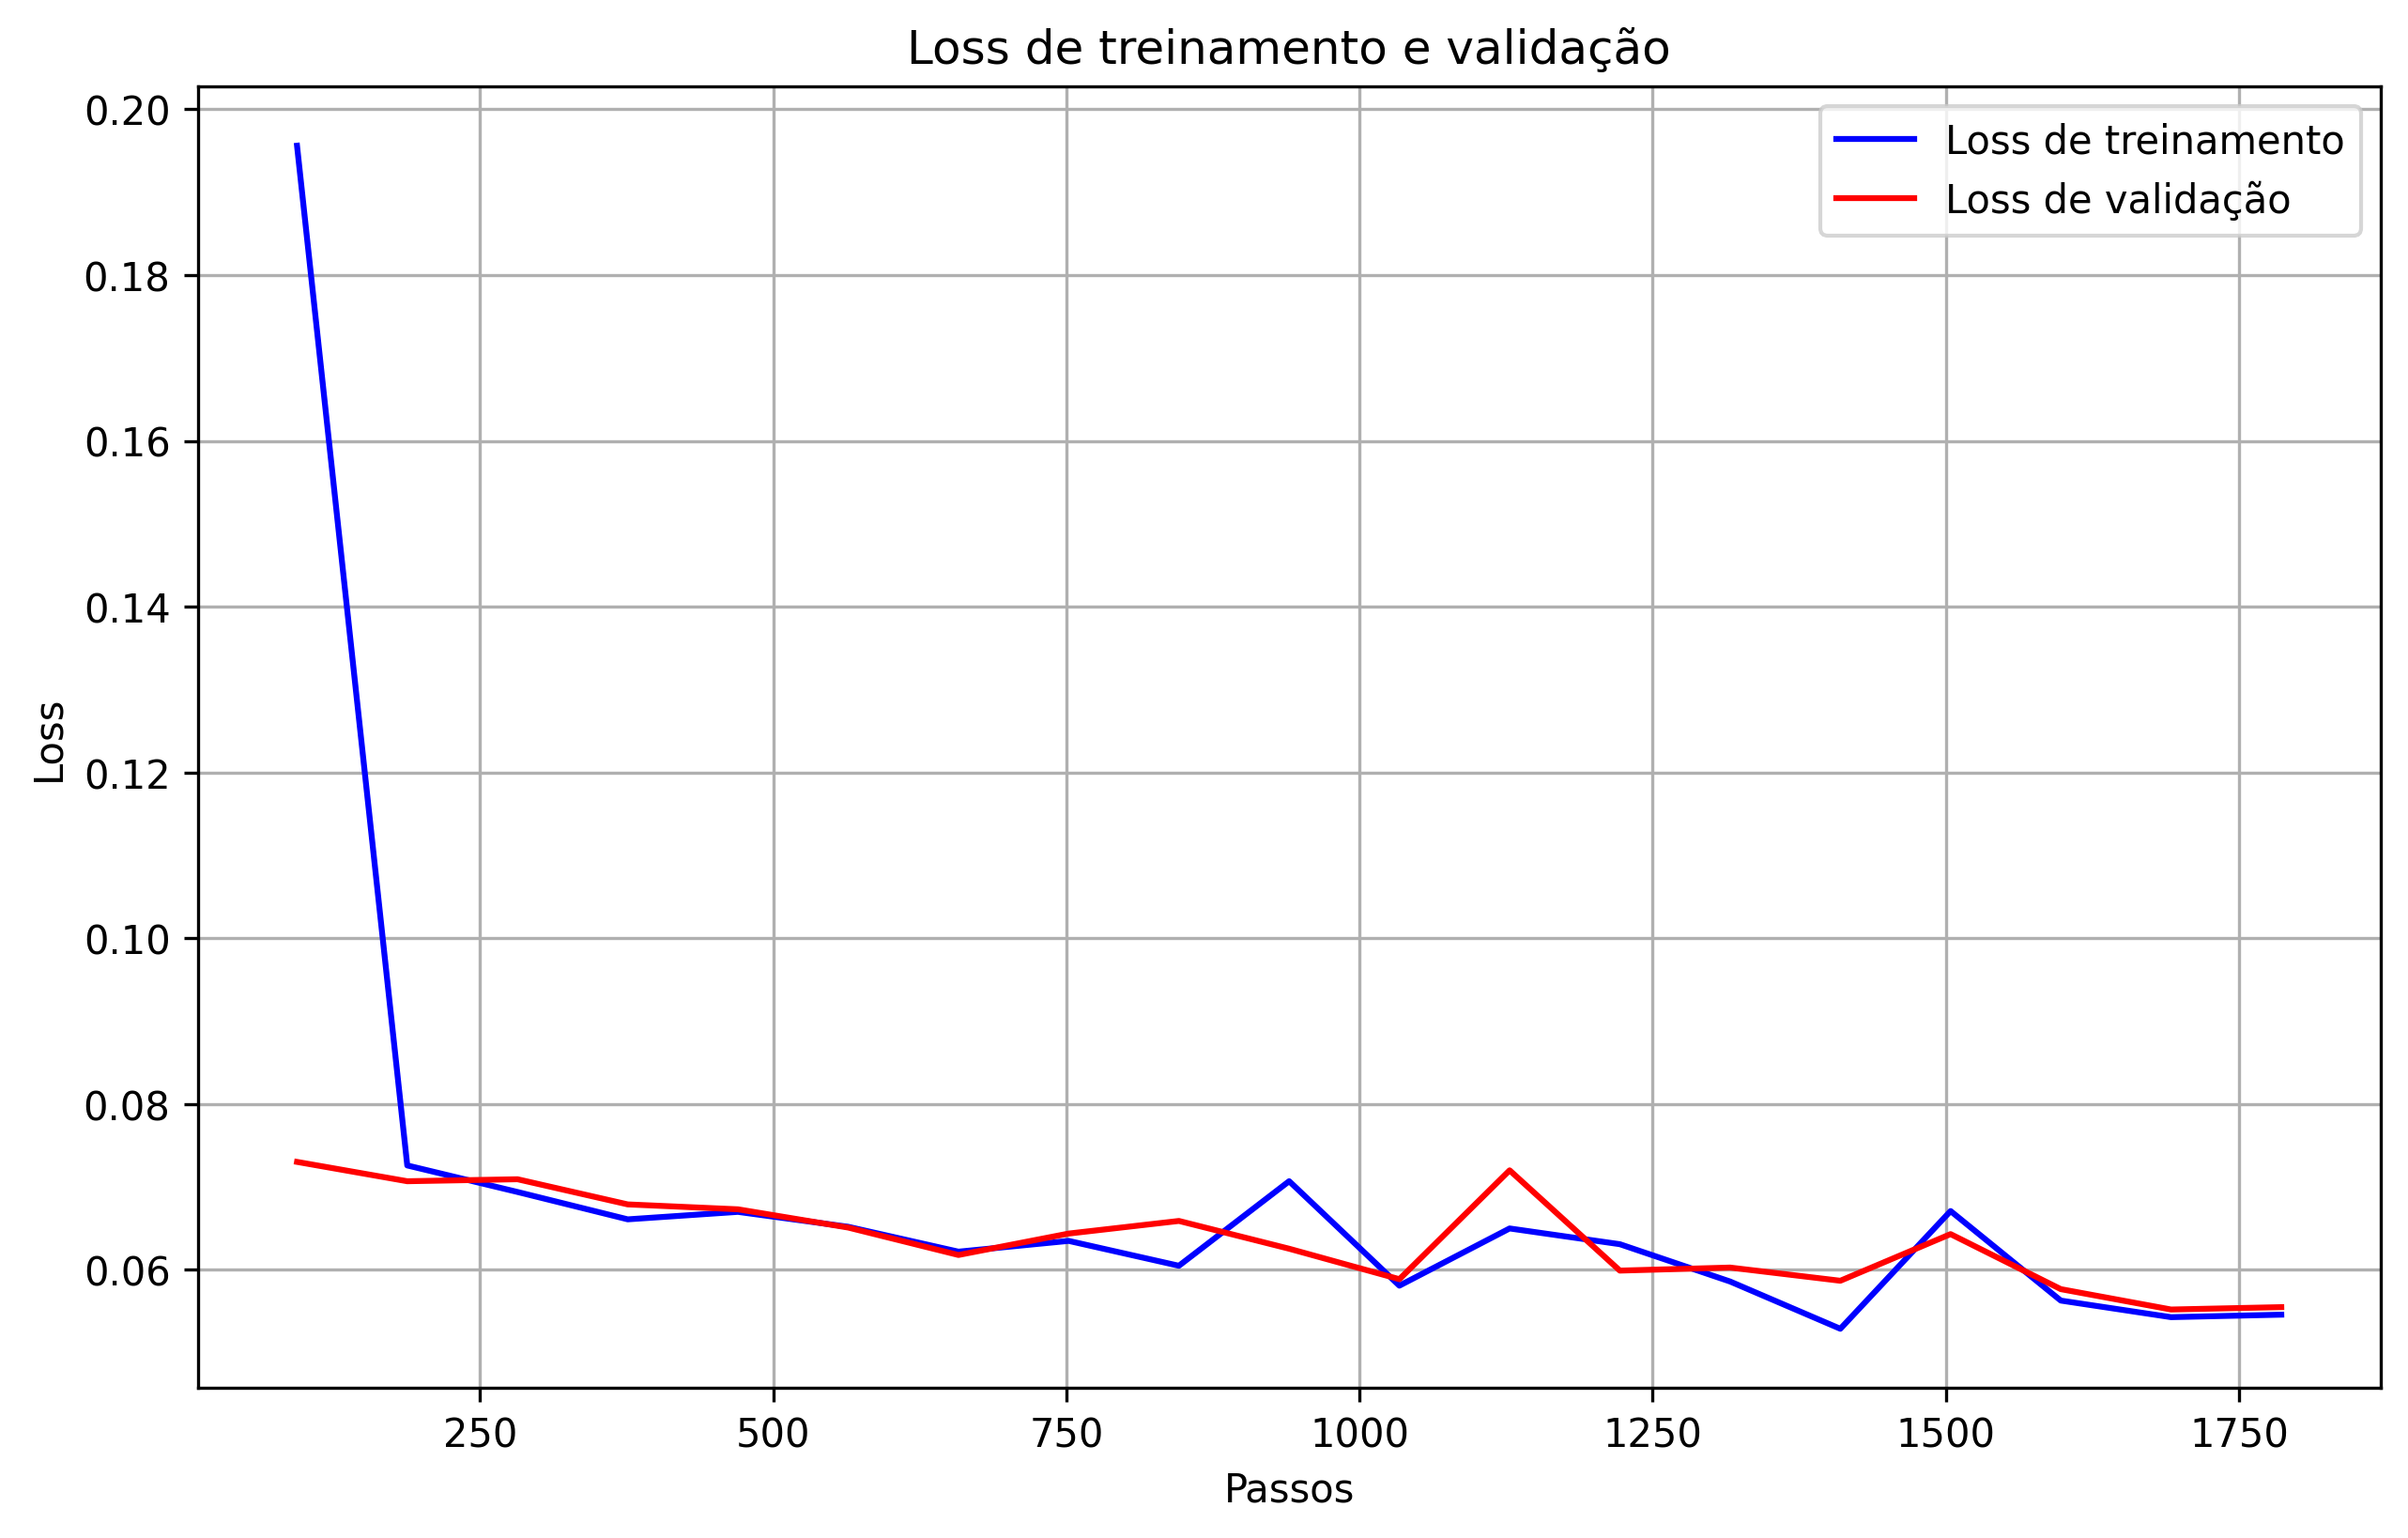
\includegraphics[width=0.725\columnwidth,keepaspectratio]{images/loss_qlora_5000.png}
    \caption{\small \textit{Loss} de treinamento e validação para o \ac{QLoRA} com 5000 amostras. Fonte: Autoria própria.}
    \label{fig:loss_qlora_5000}
\end{figure}

\clearpage

\begin{figure}[ht]
    \centering
    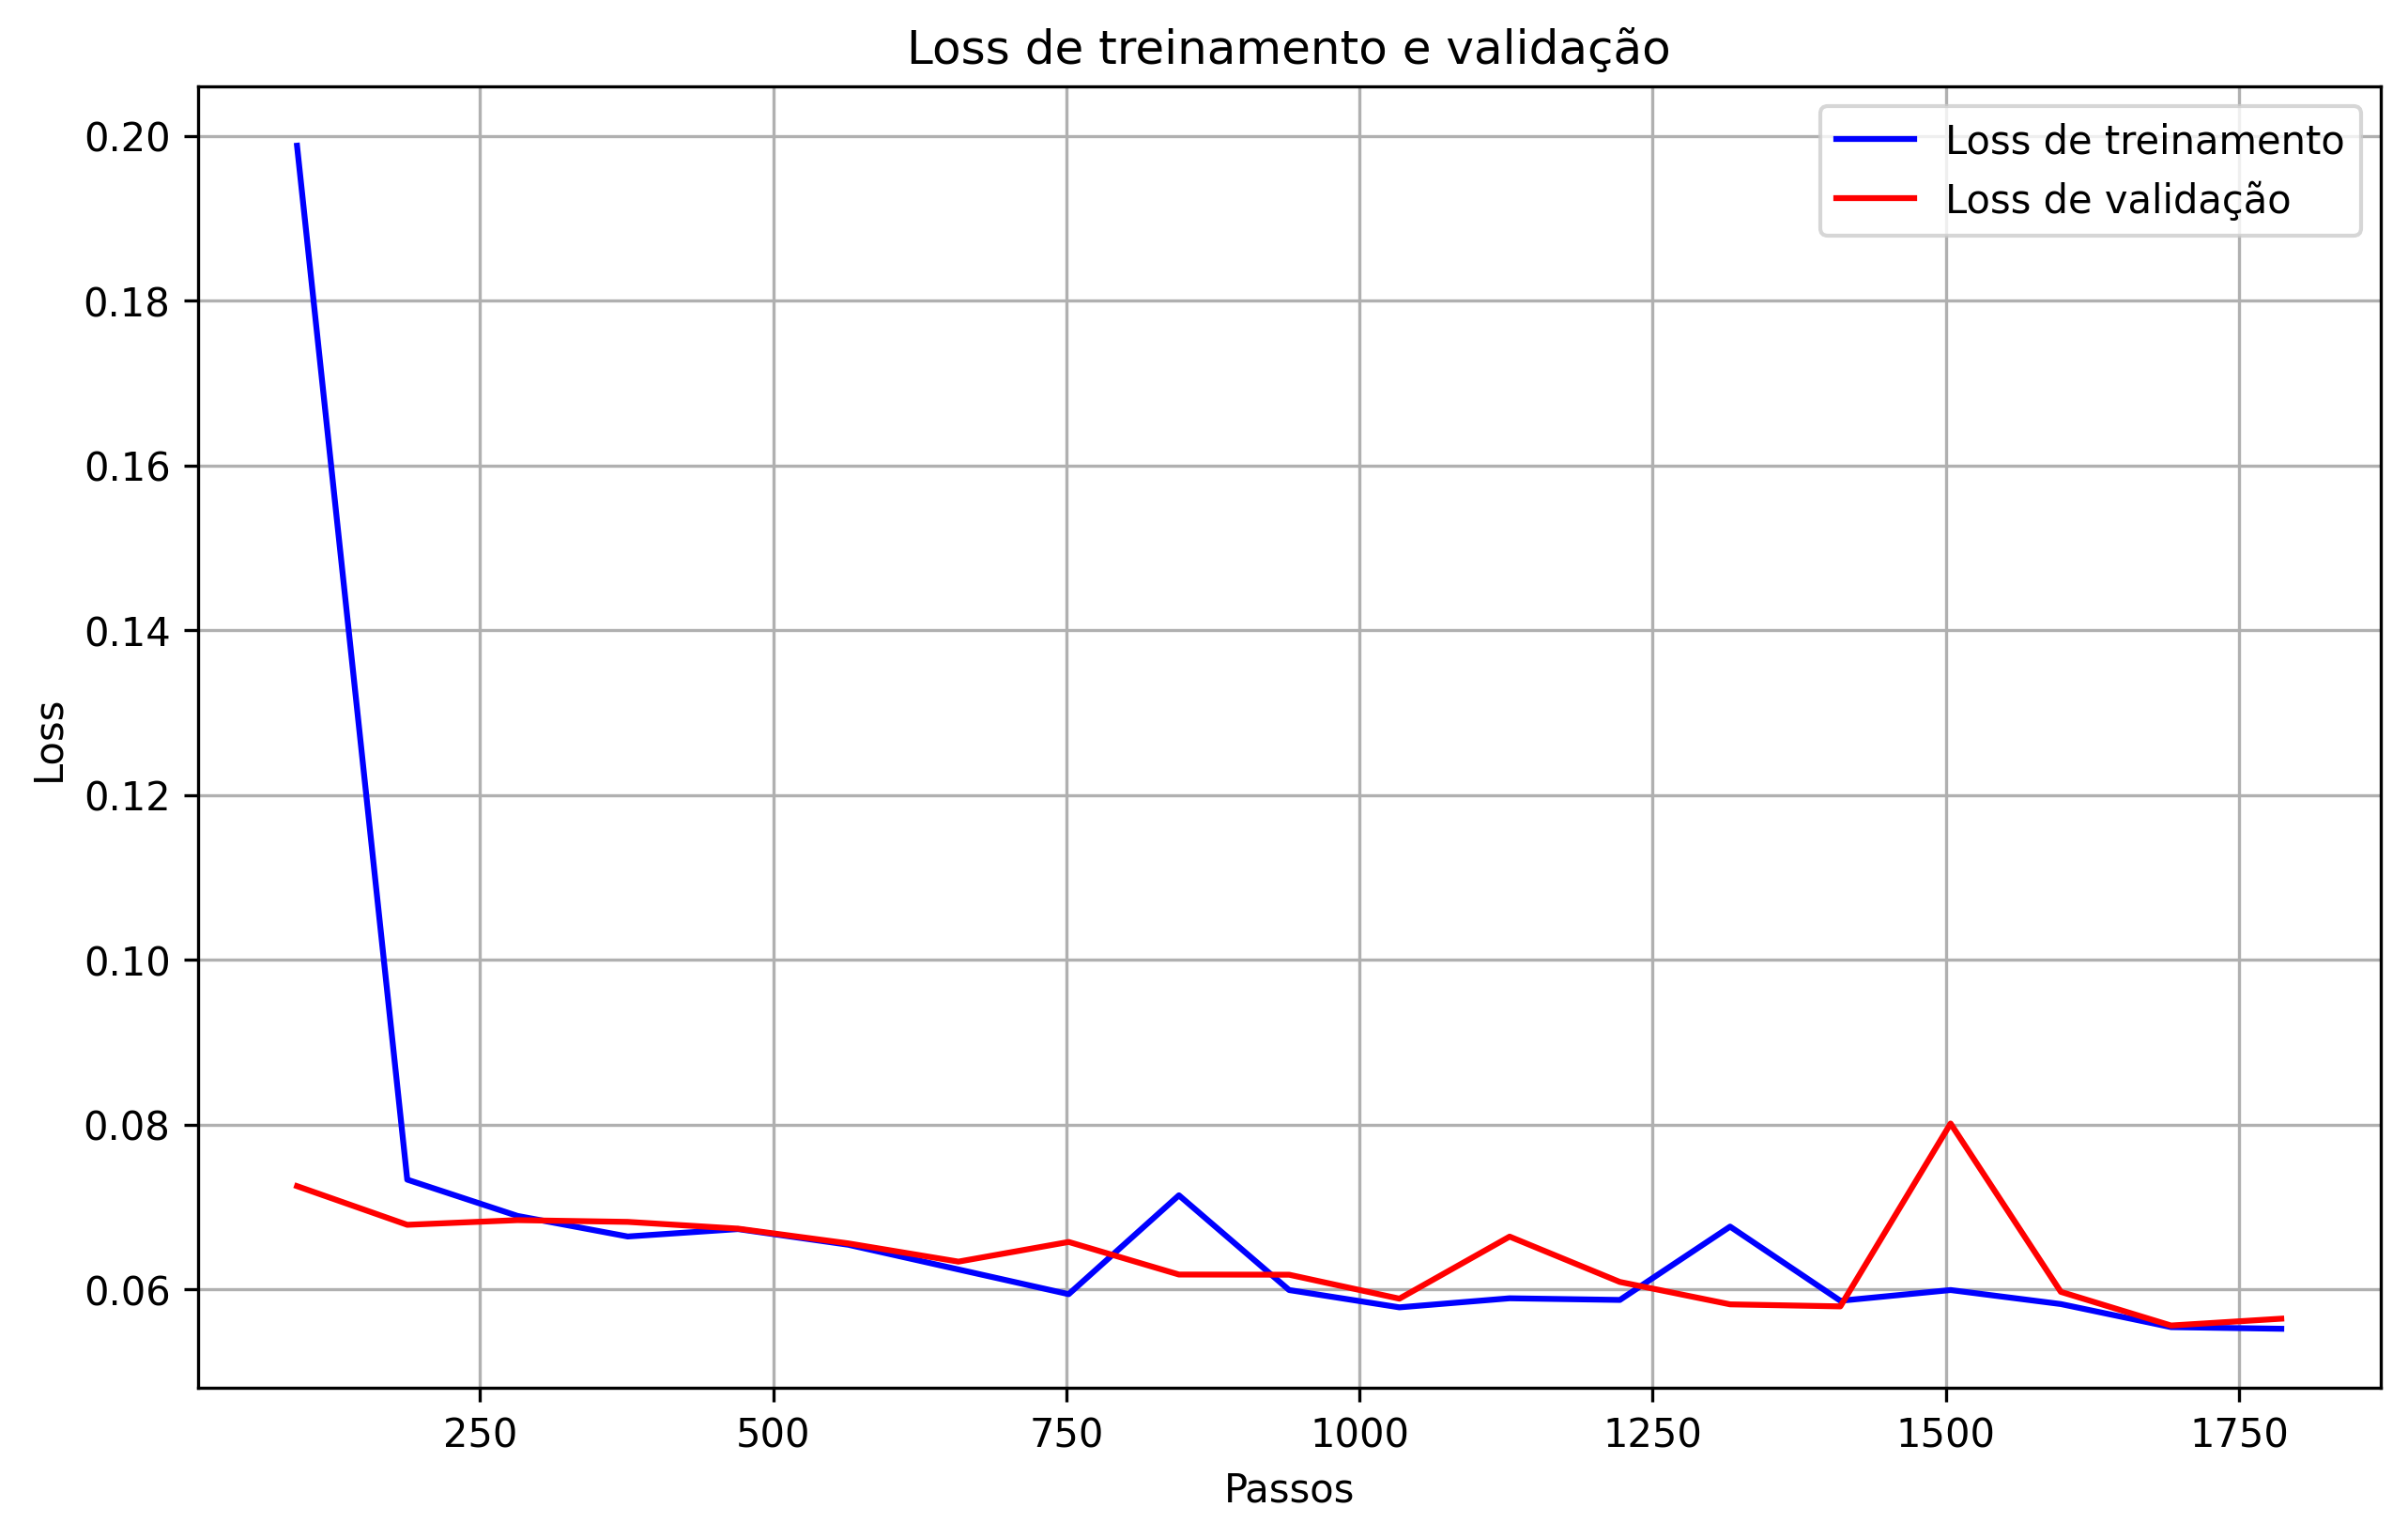
\includegraphics[width=0.725\columnwidth,keepaspectratio]{images/loss_lora_5000.png}
    \caption{\small \textit{Loss} de treinamento e validação para o \ac{LoRA} com 5000 amostras. Fonte: Autoria própria.}
    \label{fig:loss_lora_5000}
\end{figure}

\begin{figure}[ht]
    \centering
    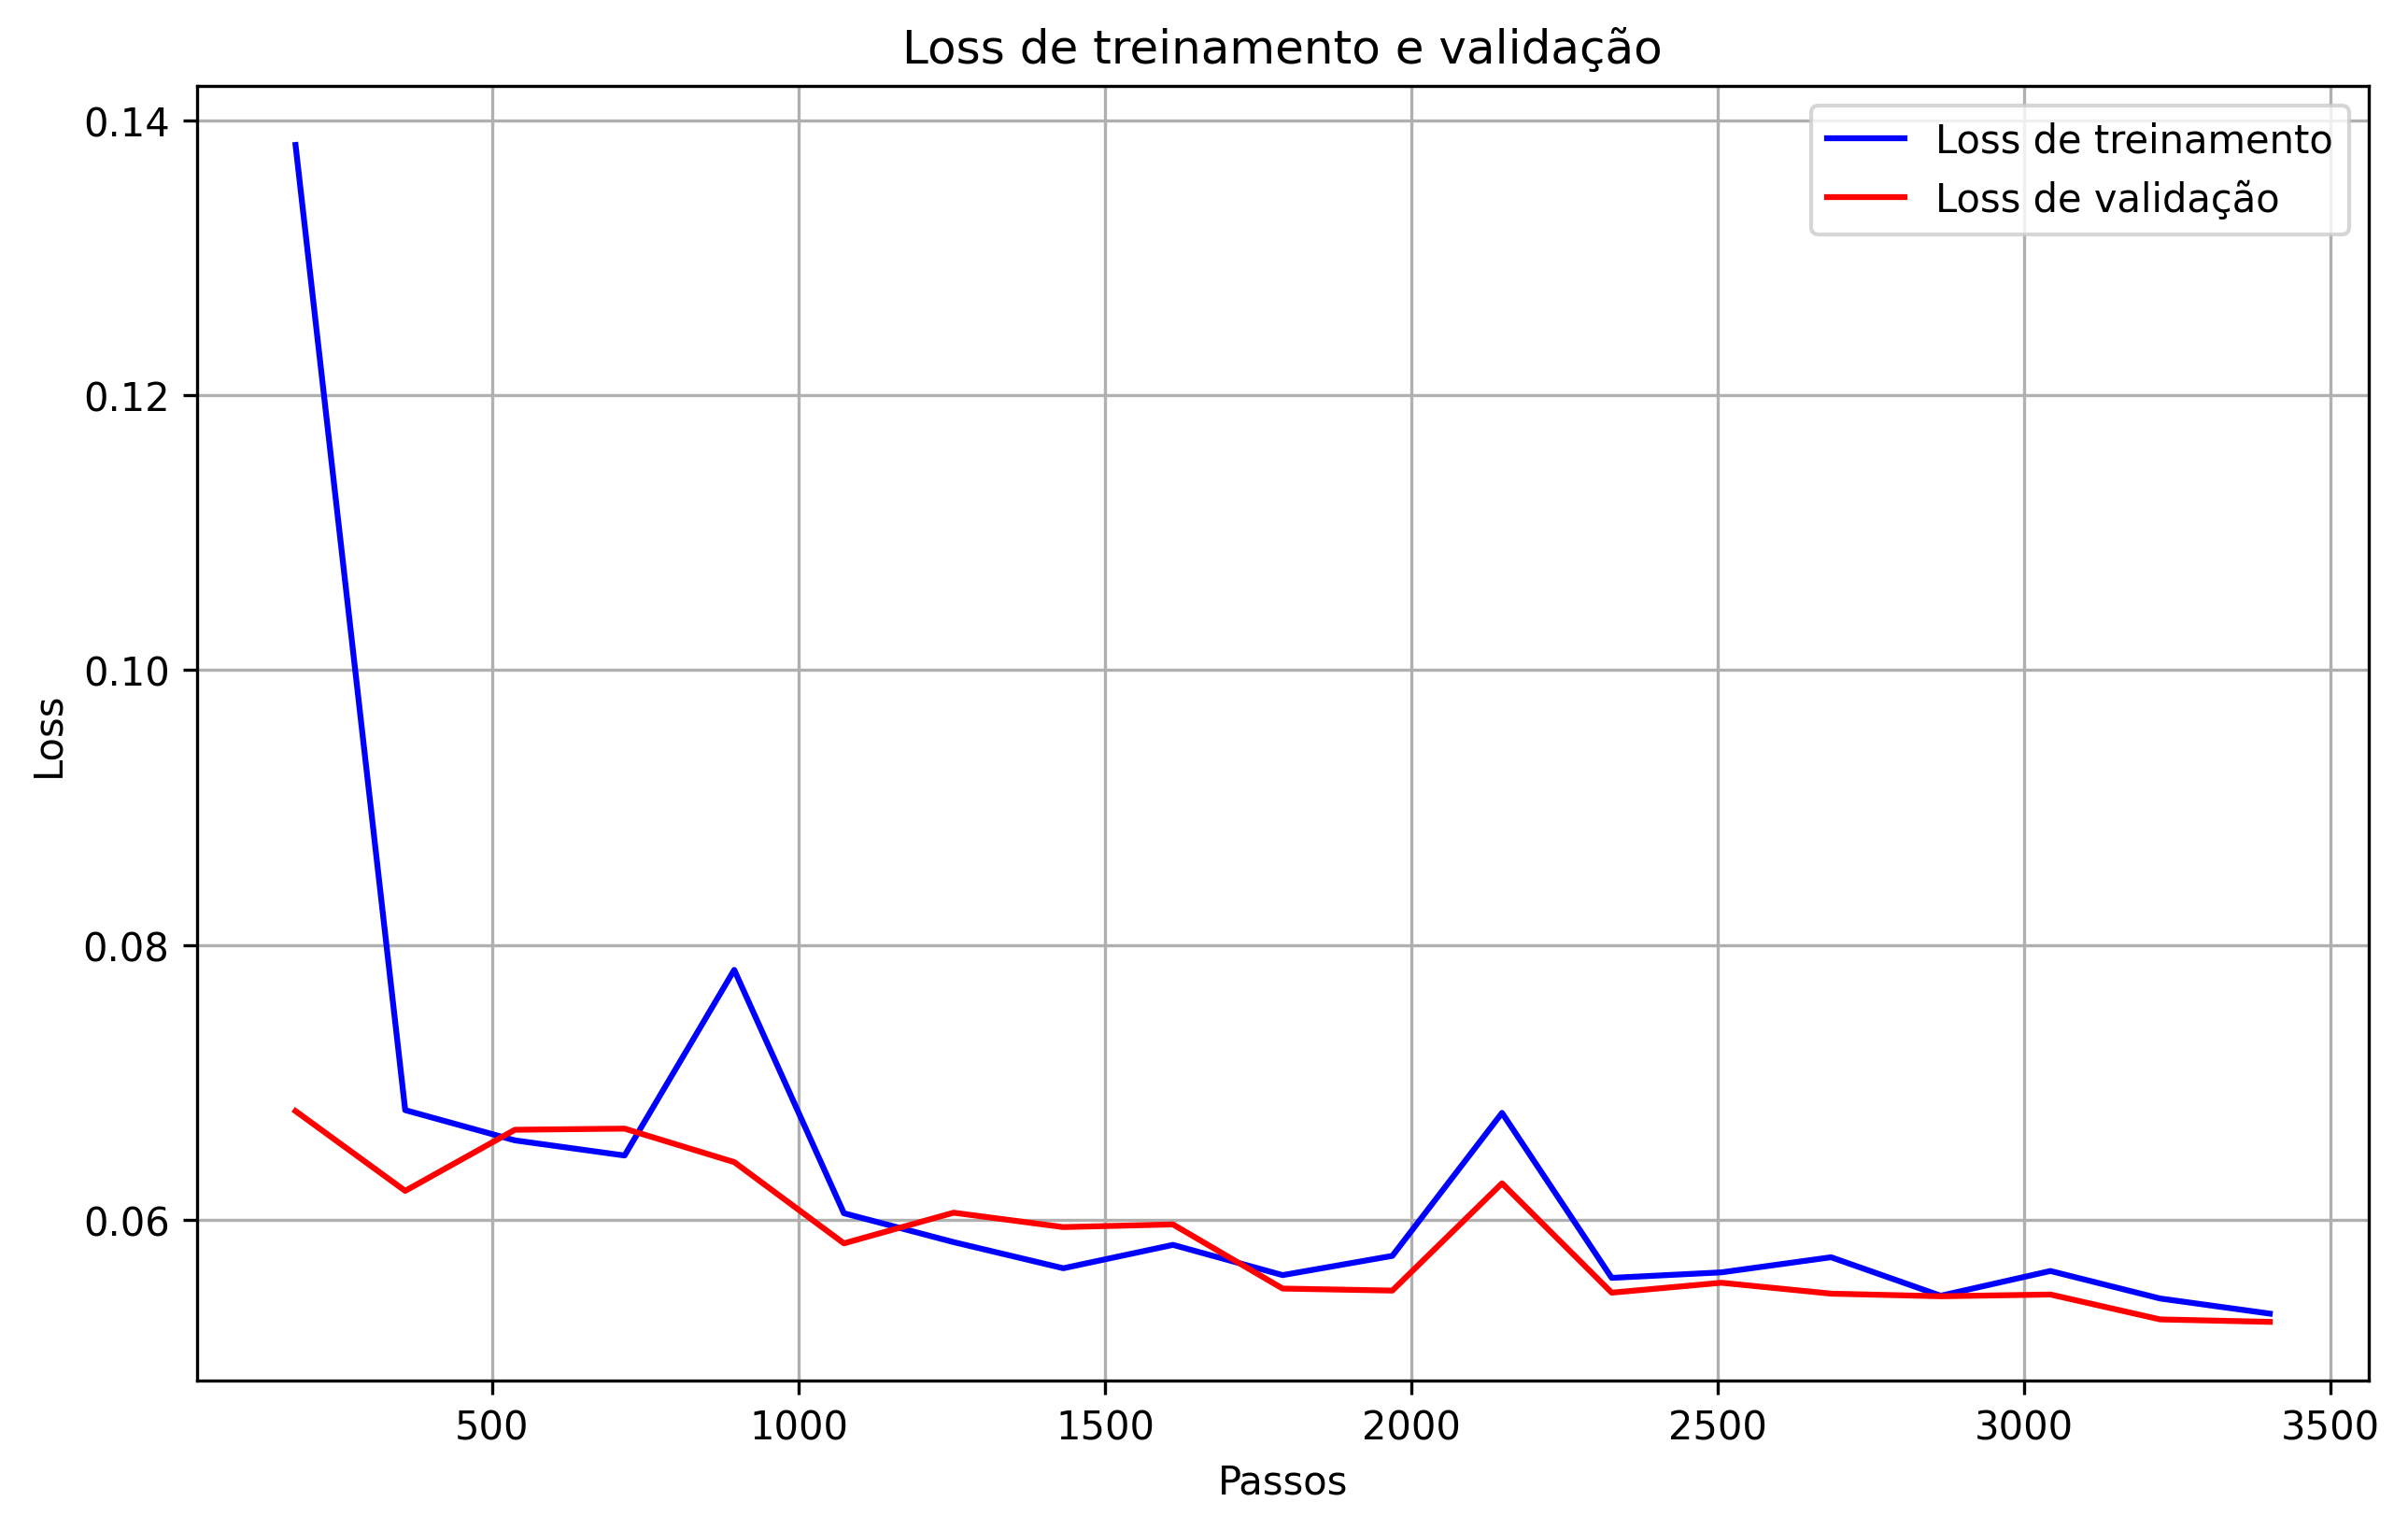
\includegraphics[width=0.725\columnwidth,keepaspectratio]{images/loss_qlora_9500.png}
    \caption{\small \textit{Loss} de treinamento e validação para o \ac{QLoRA} com 9500 amostras. Fonte: Autoria própria.}
    \label{fig:loss_qlora_9500}
\end{figure}

\subsection{Análise dos treinamentos}

A vantagem no baixo gasto de memória do \ac{QLoRA} se torna evidente com os treinamentos, usando em média 1,8 vezes menos memória que o \ac{LoRA}. Observa-se também
que as configurações de \textit{fine-tuning} usadas no treinamento com 5000 e 9500 amostras levaram a uma maior instabilidade no \textit{loss} do longo dos passos.

\section{Testes}

Os testes se consistiram em uma série de perguntas aos modelos, em que foram usadas duas modalidades de pergunta, uma livre e outra fechada. Na pergunta livre o
\textit{prompt} é definido como:

\begin{dialogue}
    \speak{Usuário} \textit{Classify the skin lesion in the image. \textbf{<imagem>}}
\end{dialogue}

Já na pergunta fechada, o objetivo é que o modelo informe apenas o nome da doença com base nas opções possíveis do conjunto de dados, sendo que o \textit{prompt} usado é:

\begin{dialogue}
    \speak{Usuário} \textit{Classify the skin lesion in the image. Say only the name of the disease and nothing else. The diseases to be classified are: melanocytic Nevi,
        melanoma, benign keratosis-like lesions, basal cell carcinoma, actinic keratoses, vascular lesions and dermatofibroma.\textbf{<imagem>}}
\end{dialogue}

Foram feitas 100 perguntas livres e 1000 perguntas fechadas para cada modelo treinado e para o \ac{LLaMA}-3.2-11B-Vision-Instruct na versão normal e na quantizada. As
imagens utilizadas vieram da seção de teste do conjunto de dados. A \textit{temperatura}, uma variável que define a previsibilidade do modelo, foi definida como 0,1 para
que as respostas fossem mais precisas. 

\section{Análise dos resultados parciais}
